\section{Decoder (Kim + William)}

\subsection{Synchronisation}
At the decoding end of the system, a pair of I and Q signals will be received from the modulation group. Here, the system will look for the ASM and use this to separate the frames from each other and identify the IQ signals as either inverted or correct. If they’re inverted, they will have to be corrected before being sent to the next box.

In case the ASM is missing (isn't where it is expected to be), a search for another ASM starts.  When an ASM at an alternative position has been found, this position will be used to find the next ASM\. Here, the system will simply look a frame-size ahead. In case two ASMs are found with a correct distance between them (matching a the size of a frame), the system will be set to a "stable" state and further ASMs are expected to found periodically.

\subsection{Error correction}
When using (64,57,4) extended Hamming code, one error can be corrected and two error can be detected in each row and column. In the error correction process, these errors will first be fixed by row and then by column.

\begin{figure}[h!]
  \centering
  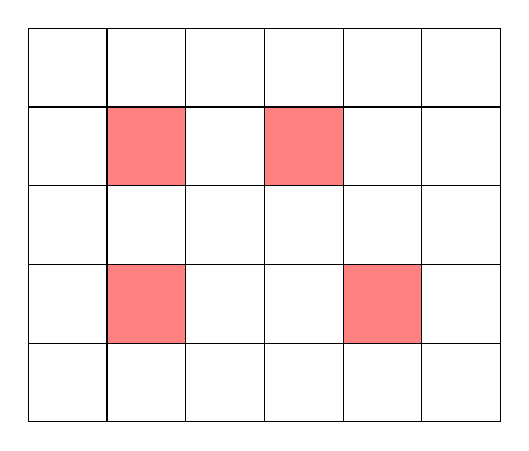
\begin{tikzpicture}
    \fill[color=red!50] (1,1) rectangle (2,2);
    \fill[color=red!50] (1,3) rectangle (2,4);
    \fill[color=red!50] (3,3) rectangle (4,4);
    \fill[color=red!50] (4,1) rectangle (5,2);
    \draw[step=1cm] (0,0) grid (6,5);
  \end{tikzpicture}
  \caption{Solvable error case (boxes marked with red represents errors)}
  \label{fig:error-case-1}
\end{figure}

To enhance the level of error correction, the system will keep fixing errors horizontal and vertical in the frame until no more errors can be corrected. With the case seen in Figure~\ref{fig:error-case-1}, it would be impossible the correct all four errors if the system were to only correct the errors first horizontal and then vertical. But by correcting the errors first horizontal and vertical and then horizontal again, all four errors will be corrected. This will ensure that most errors that occur in a pair in a single row or column will be corrected.

\begin{figure}[h!]
  \centering
  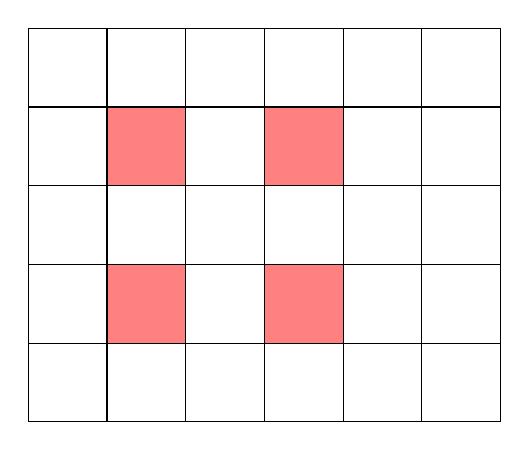
\begin{tikzpicture}
    \fill[color=red!50] (1,1) rectangle (2,2);
    \fill[color=red!50] (1,3) rectangle (2,4);
    \fill[color=red!50] (3,3) rectangle (4,4);
    \fill[color=red!50] (3,1) rectangle (4,2);
    \draw[step=1cm] (0,0) grid (6,5);
  \end{tikzpicture}
  \caption{Unsolvable error case (boxes marked with red represents errors)}
  \label{fig:error-case-2}
\end{figure}

\subsection{Deframing}
During the deframing process, the audio and video data is located in each frame based on the pointers and the corresponding bit data is sent on to the audio and video group.

\subsection{Audio \& video}
The audio and video stream is sent along with a clock and a receipt which tells the receiver whether or not it is real data, or just dummy data, that has been sent. The dummy data is used when there isn't any real data present, but something is still needed to be sent at the clock cycle.
